%%%%%%%%%%%%%%%%%%%%%%%%%%%%%%%%%%%%
%%                                %%
%%       Messages, Priorities     %%
%%         Groups, Nodegroups     %%
%%%%%%%%%%%%%%%%%%%%%%%%%%%%%%%%%%%%
\subsection[Messages]{Messages}

\begin{frame}[fragile]
  \frametitle{Messages}
  \begin{itemize}
    \item A message is a struct | class that inherits from a system-defined class
    \item It provides explicit control for the application over allocation, reuse, and scope
    \begin{itemize}
      \item Marshalled parameters go out of scope at the end of the entry method
      \item Messages are explicitely deleted by the application
    \end{itemize}
    \item In the ``.ci'' file:
      \begin{itemize}
         \begin{lstlisting}
message MyMsgType;
         \end{lstlisting}
         \item The interface translator produces code for a class named
         \begin{lstlisting}
CMessage_MyMsgType
         \end{lstlisting}
      \end{itemize} 
      \item In the ``.h'' or ``.C'' file, define
      \begin{lstlisting}
class MyMsgType : public CMessage_MyMsgType {...};
      \end{lstlisting}
  \end{itemize}
\end{frame}

\begin{frame}[fragile]
  \frametitle{Variable-Size Messages}
  \framesubtitle{Declaration}
  \begin{itemize}
    \item In the “.ci” file, declare the name and type of variable length arrays
    \begin{lstlisting}
message MyVarsizeMsg {
  int arr1[];
  MyStruct arr2[];
};
    \end{lstlisting}
    \item Corresponding definition in .h file
    \begin{lstlisting}
class MyVarsizeMsg : public CMessage_MyVarsizeMsg {
  // variable-length arrays
  int *arr1;
  MyStruct *arr2;
};
    \end{lstlisting}
  \end{itemize}
\end{frame}

\begin{frame}[fragile]
  \frametitle{Variable-Size Messages}
  \framesubtitle{Allocation}
  \begin{itemize}
    \item Use optional arguments in brackets for variable size arrays
    \item Sizes used in-order to allocate arrays
  \end{itemize}
  \begin{lstlisting}
MessageType *msgptr = new (int sz1, int sz2, ... ) 
                      MessageType(constructor arguments);

MyVarsizeMsg *msg = new (10,  7)        
                    MyVarsizeMsg(<constructor args>);
  \end{lstlisting}
  \begin{itemize}
    \item This defines arr1 to be an integer array of length 10, and arr2 to be MyStruct array of length 7
    \item Charm forces them to be in a contiguous memory segment
  \end{itemize}
\end{frame}

\begin{frame}[fragile]
  \frametitle{Variable-Size Messages}
  \framesubtitle{Allocation by Array}
  \begin{itemize}
    \item Alternatively, one can use an array of integers to specify size of variable arrays
    \begin{lstlisting}
int sizes[2];
sizes[0] = 10; sizes[1] = 7
MyVarsizeMsg *msg = new (sizes)        
                    MyVarsizeMsg(<constructor args>);
    \end{lstlisting}
    \item Messages passed to Charm belong to Charm – deleted or reused by Charm after sending
    \item Message delivered by Charm belongs to user – can be reused or deleted
  \end{itemize}
\end{frame}

\begin{frame}[fragile]
  \frametitle{Changing Message Order}
  \begin{itemize}
    \item To set the queueing strategy for execution of received events
    \begin{itemize}
      \item \code{void CkSetQueueing(MsgType message, int queueingtype)}
    \end{itemize}
    \item Following queueing types can be set
    \begin{itemize}
      \item \code{CK\_QUEUEING\_FIFO} : FIFO ordering (default)
      \item \code{CK\_QUEUEING\_LIFO} : LIFO ordering
      \item \code{CK\_QUEUEING\_IFIFO} : FIFO ordering with integer priority
      \item \code{CK\_QUEUEING\_ILIFO} : LIFO ordering with integer priority
      \item \code{CK\_QUEUEING\_BFIFO} : FIFO ordering with bitvector priority
      \item \code{CK\_QUEUEING\_BLIFO} : LIFO ordering with bitvector priority
      \item \code{CK\_QUEUEING\_LFIFO} : FIFO ordering with long integer priority
      \item \code{CK\_QUEUEING\_LLIFO} : FIFO ordering with long integer priority
    \end{itemize}
 \end{itemize}
\end{frame}

\begin{frame}[fragile]
  \frametitle{Changing Message Order}
  \framesubtitle{Storage of Priority}
  \begin{itemize}
    \item If using integer/long integer/bit vector priorities, one needs to reserve memory in messages to store priority
     \begin{itemize}
       \item Last size argument (in bits) in brackets to new
     \end{itemize}
    \begin{lstlisting}
MyVarsizeMsg *msg = new (10,7, 8*sizeof(int))         
                    MyVarsizeMsg(<constructor args>);

*(int*)CkPriorityPtr(msg) = prio; // set priority

int* prioMsg = CkPriorityPtr(msg);  // get priority
    \end{lstlisting}
    \item LIFO/FIFO used to break ties if multiple messages have same priority
  \end{itemize}
\end{frame}

\begin{frame}[fragile]
  \frametitle{Changing Message Order}
  \framesubtitle{Marshalled Messages}
  \begin{itemize}
    \item queueingtype can be set for CkEntryOptions , which is passed to an entry method invocation as the optional last parameter
    \begin{lstlisting}
CkEntryOptions opts1, opts2;
opts1.setQueueing(CK_QUEUEING_FIFO);
opts2.setQueueing(CK_QUEUEING_LIFO);
chare1.entry_name(arg1, arg2, opts1);
chare2.entry_name(arg1, arg2, opts2);
    \end{lstlisting}
    \item \code{opts.setPriority(prio\_t integerPrio);} set integer priorities
    \item \code{opts.setPriority(int prioBits,const prio\_t *prioPtr)}  set bit vector priority using prioPtr
  \end{itemize}
\end{frame}

\begin{frame}[fragile]
  \frametitle{Customizing Message Handling}
  \begin{itemize}
    \item By default, Charm generates following three methods for each Message class
    \begin{itemize}
      \item \code{static void* alloc(int msgn, size\_t sz, int* arr, int prio);}
      \item \code{static void* pack(mtype*);}
      \item \code{static mtype* unpack(void*);}
    \end{itemize}
   \item One may override these with their own implementation
   \begin{itemize}
     \item Useful for non-contiguous allocation
     \item \code{alloc} is invoked when \code{new} is called
     \item \code{pack} and \code{unpack} are for sending/receiving the message, and should be according to alloc
     \item Optimized \code{pack}/\code{unpack} using application knowledge
   \end{itemize}
  \end{itemize}
\end{frame}

\begin{frame}[fragile]
  \frametitle{Custom-packed Messages}
  \begin{itemize}
    \item How to pack messages that contain pointers to structures such as trees or graphs?
    \begin{itemize}
       \item i.e. pointers leading to pointers,
       \item Manual section: 10.1.3.1
    \end{itemize}
  \end{itemize}
\end{frame}

\begin{frame}[fragile]
  \frametitle{Messages}
  \framesubtitle{Motivation Summary}
  \begin{itemize}
    \item Avoids extra copy
    \item Can be custom packed
    \item Reusable
    \item Useful for transfer of complex data structures
  \end{itemize}
\end{frame}
\subsection[Groups]{Groups and NodeGroups}
\begin{frame}[fragile]
  \frametitle{Groups}
  \begin{itemize}
    \item Like a chare-array with one chare per PE
    \item In .ci file, 
    \begin{lstlisting}
group ExampleGroup {
  // Interface specifications as for normal chares
  // For instance, the constructor ...
  entry ExampleGroup(parameters1);
  // ... and an entry method
  entry void someEntryMethod(parameters2);
};
    \end{lstlisting}
    \item No difference in .h and .C file definitions
  \end{itemize}
\end{frame}

\begin{frame}[fragile]
  \frametitle{Groups}
  \framesubtitle{Example use}
  \begin{itemize}
    \item  One can obtain pointer to the local group member using groupProxy.ckLocalBranch()
    \begin{itemize}
      \item Access the local member as a regular C++ object
    \end{itemize}
   \item Consider a case:
   \begin{itemize}
      \item each chare on a processor performs a task and wants to pass some information to the mainchare
      \begin{itemize}
         \item Assume reduction is not feasible
      \end{itemize}
      \item One way is to directly send this information to mainchare from every chare (too many messages)
      \item Alternatively, each chare may deposit the information to the local branch of a group
      \begin{itemize}
        \item How to obtain a pointer to local branch? Manual 8.1.3
        \item \code {Gclass * g = grpProxy.ckLocalBranch();}
        \item \code{g} is a regular pointer to a C++ object
        \item Group member can pass this information to the mainchare after optional pre-processing when all chares have deposited 
      \end{itemize}
    \end{itemize}
  \end{itemize}
\end{frame}

\begin{frame}[fragile]
  \frametitle{Sharing data between chares using groups}
  \begin{itemize}
  \item Often applications exhibit data reuse across chares on a PE
  \item Exploit this using Groups
  \item Pattern:
    \begin{itemize}
    \item Group local branch ``owns'' data, not chares
    \item Chares request group for data
    \item Via (local entry) methods defined on group
    \end{itemize}
  \end{itemize}
\end{frame}

\begin{frame}[fragile]
  \frametitle{Sharing data between chares: an example}
  \begin{itemize}
    \item Barnes-Hut type long-range $N$-body simulation
    \item C1, C2, C3 request similar data from owner of some subvolume, C4
  \end{itemize}
  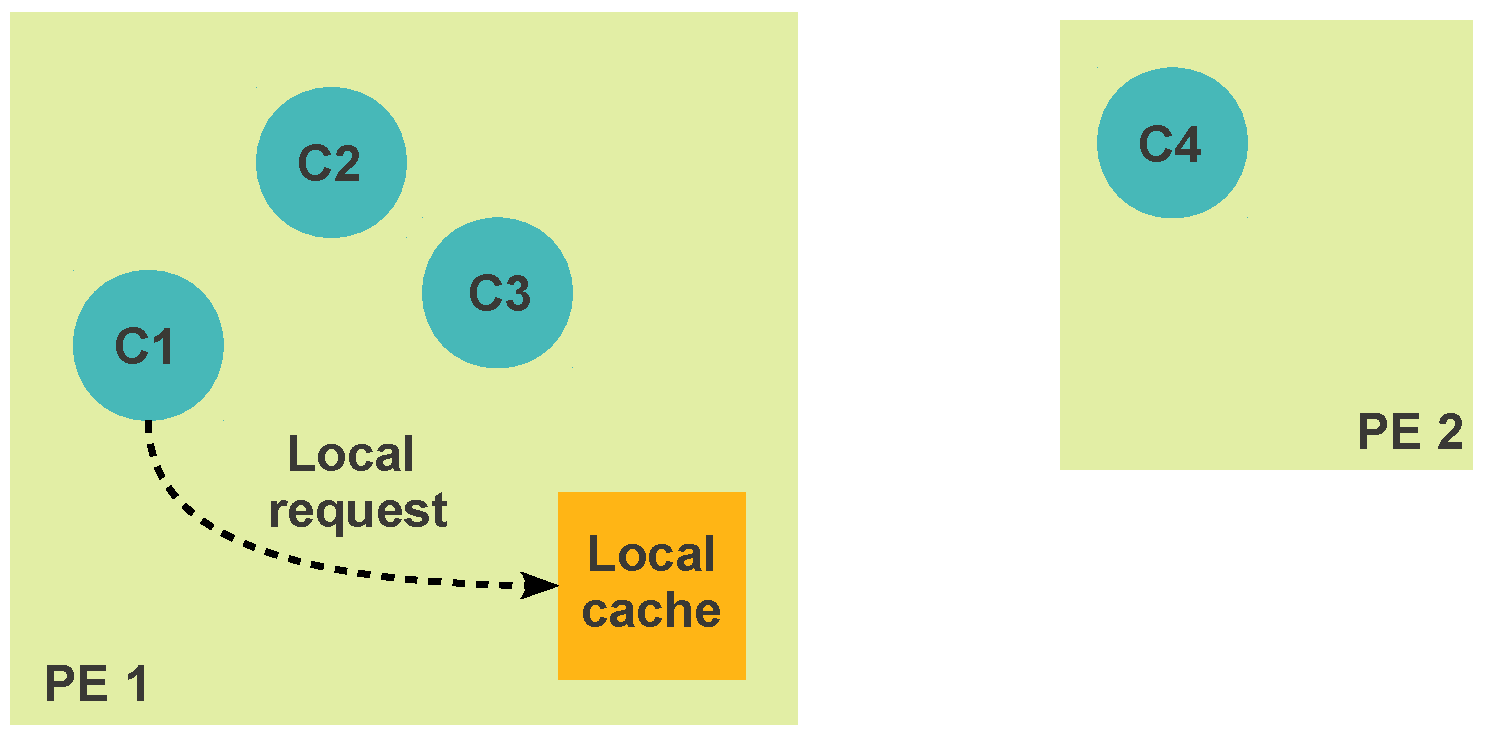
\includegraphics[width=\textwidth]{figures/advancedOpts/fig4}
\end{frame}

\begin{frame}[fragile]
  \frametitle{Sharing data between chares: an example}
  \begin{itemize}
    \item First-time requests forwarded to owner of data 
  \end{itemize}
  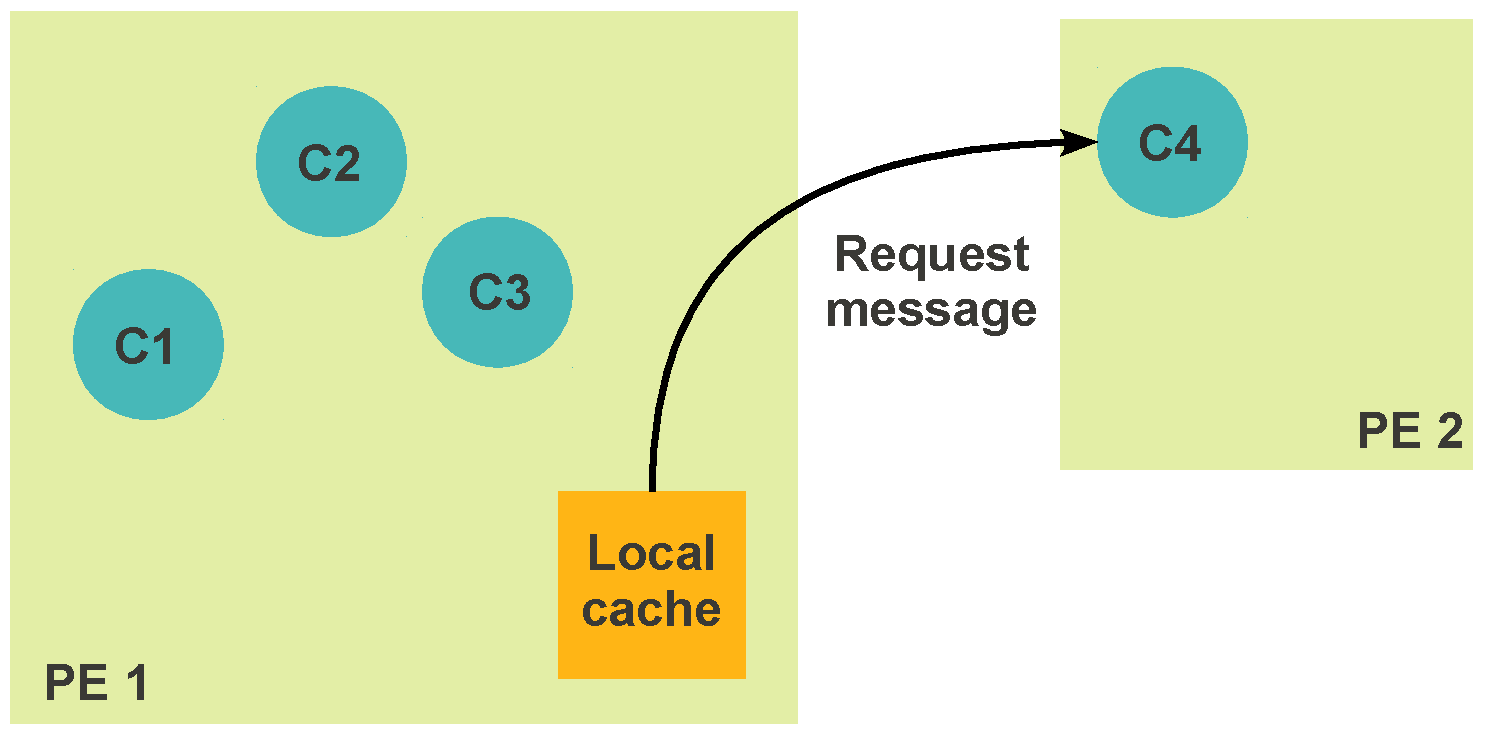
\includegraphics[width=\textwidth]{figures/advancedOpts/fig5}
\end{frame}

\begin{frame}[fragile]
  \frametitle{Sharing data between chares: an example}
  \begin{itemize}
    \item ``Duplicate'' requests do not result in messages, only local book-keeping
  \end{itemize}
  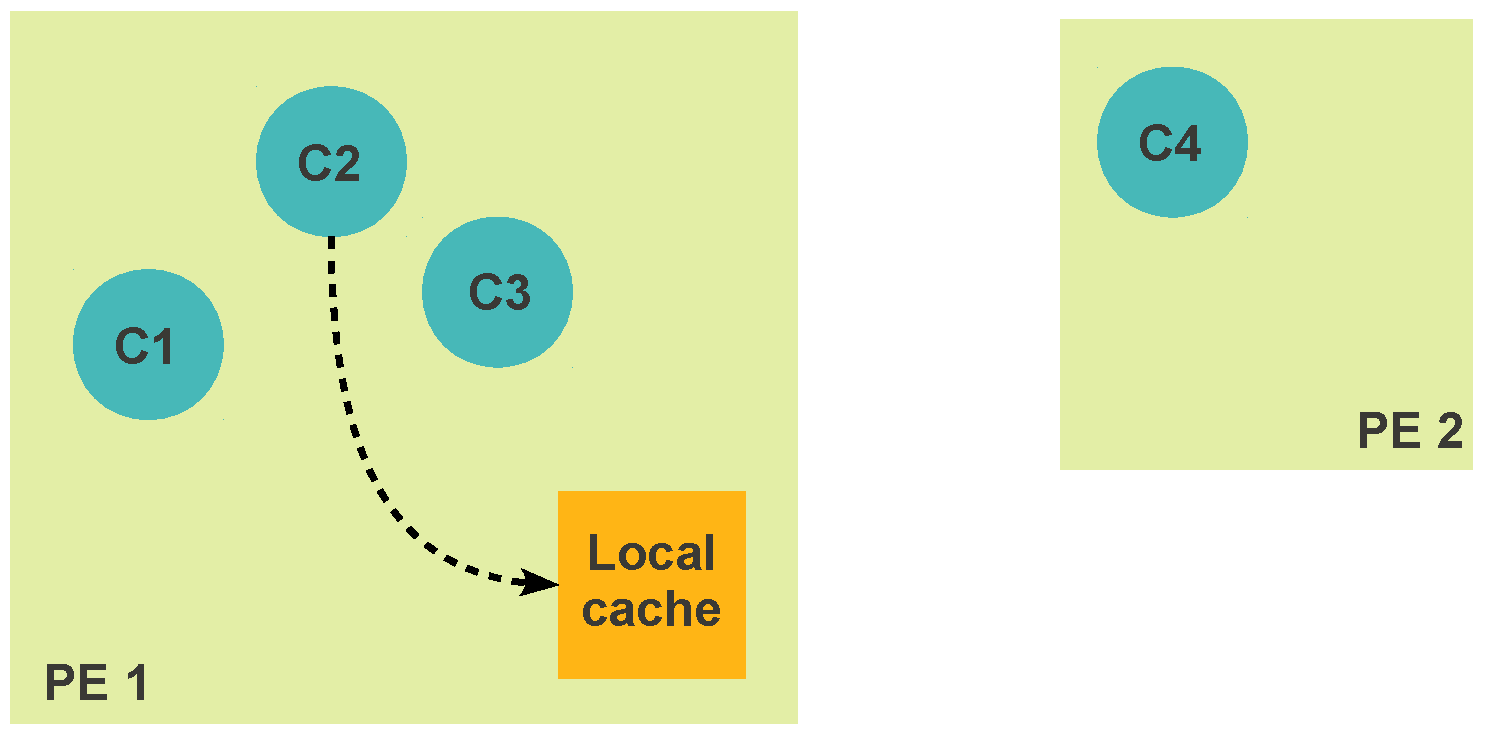
\includegraphics[width=\textwidth]{figures/advancedOpts/fig6}
\end{frame}

\begin{frame}[fragile]
  \frametitle{Sharing data between chares: an example}
  \begin{itemize}
    \item Data relayed to requestors when available on PE
  \end{itemize}
  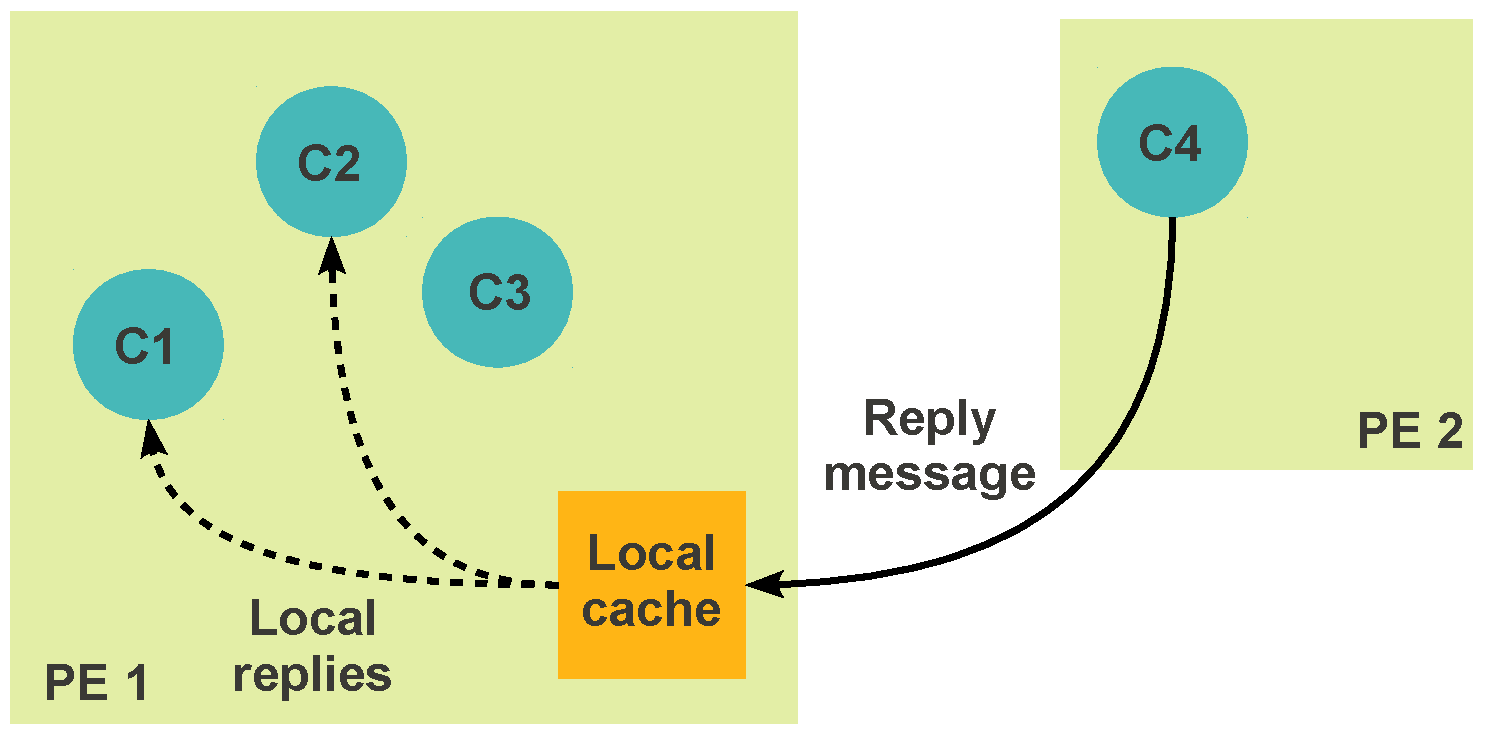
\includegraphics[width=\textwidth]{figures/advancedOpts/fig7}
\end{frame}

\begin{frame}[fragile]
  \frametitle{Sharing data between chares: an example}
  \begin{itemize}
    \item If data has already been fetched, immediately provided to requestor
  \end{itemize}
  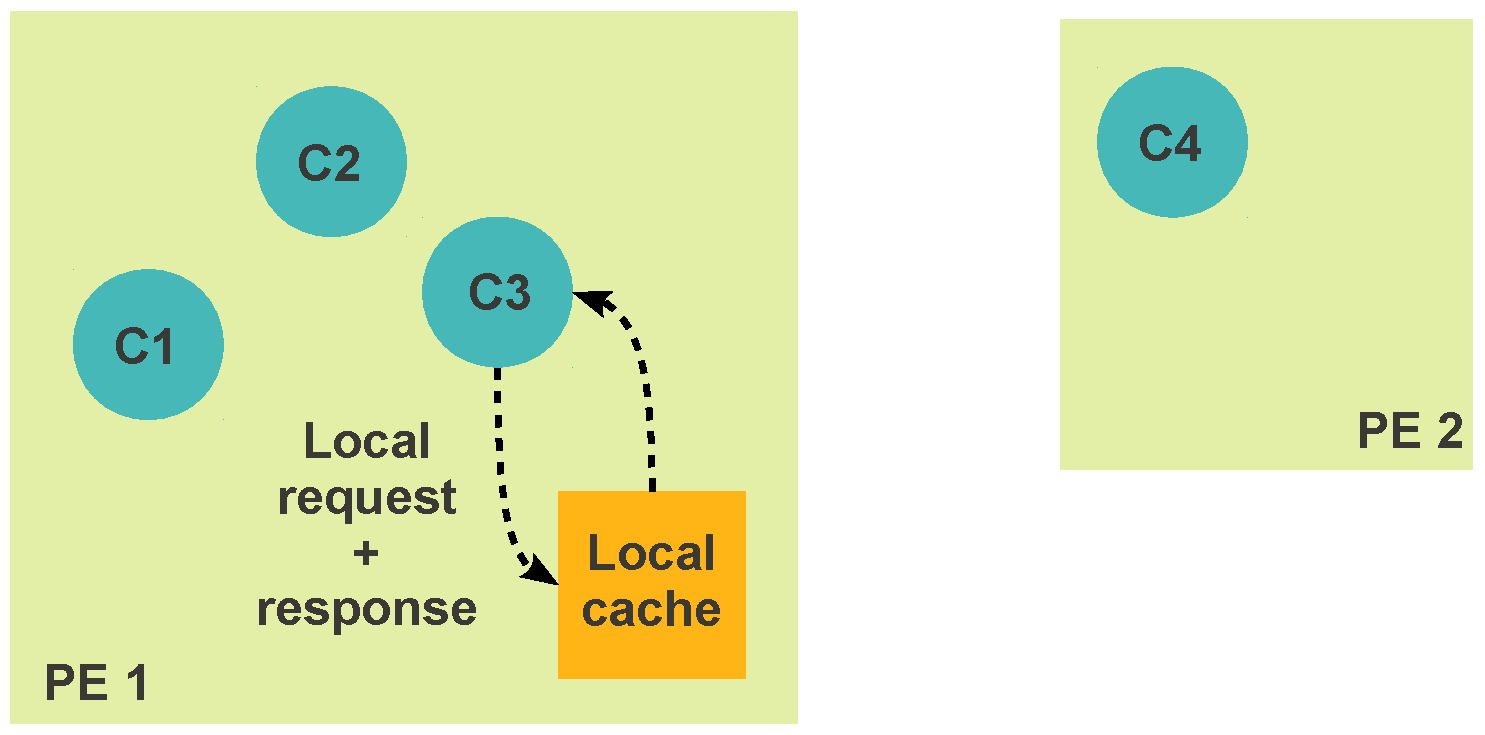
\includegraphics[width=\textwidth]{figures/advancedOpts/fig8}
\end{frame}

\begin{frame}[fragile]
  \frametitle{Node Groups}
  \begin{itemize}
    \item A chare-array with one chare per node
    \begin{itemize}
      \item In non-smp mode groups and node groups are same
    \end{itemize}
    \item No difference in .h and .C
    \item Creation and usage same as others
    \item An entry method on a node-group member may be executed on any PE of the node
    \item Concurrent execution of two entry methods of a node-group member may happen
    \begin{itemize}
      \item Use \code{[exclusive]} for entry methods which are unsuitable for reentrance safety
    \end{itemize}
  \end{itemize}
\end{frame}

\begin{frame}[fragile]
  \frametitle{Sharing data between cores with Node Groups}
  \begin{itemize}
    \item In previous example, chares on {\em same PE} shared remotely fetched data
    \item Same idea can be used to share data {\em across PEs} on same logical node
    \item {\em Node Groups}: one local branch per logical node
    \item {\bf Caution:}
    \begin{itemize}
      \item Nodegroup methods {\em not thread-safe} by default! 
      \item Use node-level locks for core synchronization
    \end{itemize}
  \end{itemize}
\end{frame}

\subsection[Entry Methods]{Entry Methods}
\begin{frame}[fragile]
  \frametitle{Customizing Entry Method Attributes}
  \begin{itemize}
    \item \code{threaded} – executed using separate thread
    \begin{itemize}
      \item each thread has a stack, and may be suspended, for sync methods or futures
      \item to set stack’s size use +stacksize $<$ size in bytes $>$
    \end{itemize}
    \item \code{sync} - returns a value
    \item \code{inline} – entry method invoked immediately if destination chare on same PE
    \begin{itemize}
      \item blocking call
    \end{itemize}
    \item \code{reductiontarget} – target of an array reduction
    \begin{itemize}
      \item Takes parameter marshaled arguments
    \end{itemize}
    \item \code{notrace} – not traced for projections
  \end{itemize}
\end{frame}

\begin{frame}[fragile]
  \frametitle{Customizing Entry Methods}
  \begin{itemize}
    \item \code{expedited} – entry method skips the priority-based message queue in Charm++ runtime (for groups)
    \item \code{immediate} - skips the message scheduling queue (for any chare array)
    \item \code{nokeep} – message belongs to Charm
    \item \code{exclusive} – mutual exclusion on execution of entry methods on node-groups 
    \item \code{python} – can be called from python scripts
  \end{itemize}
\end{frame}

